
\definecolor{cblue}{HTML}{4A90D9}
\definecolor{cgreen}{HTML}{5BAD72}
\definecolor{corange}{HTML}{E8863A}
\definecolor{cpurple}{HTML}{512E78}
\definecolor{cgray}{HTML}{7F8C8D}
\definecolor{cred}{HTML}{D9534F}

\newcommand{\snowflake}[1][0.12]{%
    \tikz[scale=#1, baseline=-0.1em, rotate=30]{
        \pgfmathsetmacro{\R}{0.35}
        \pgfmathsetmacro{\L}{0.8}
        \pgfmathsetmacro{\br}{0.3*\L}
        \pgfmathsetmacro{\blen}{0.55*\L}
        \draw[line width=0.65pt, white] (0:{\R}) \foreach \a in {60,120,...,360} {-- (\a:{\R})} -- cycle;
        \foreach \a in {0,60,...,300} {
            \draw[line width=0.65pt, line cap=round, white] (\a:{\R}) -- (\a:{\R+\L});
            \draw[line width=0.65pt, line cap=round, white] (\a:{\R+\br}) -- ++(\a+50:{\blen});
            \draw[line width=0.65pt, line cap=round, white] (\a:{\R+\br}) -- ++(\a-50:{\blen});
        }
    }%
}

\begin{tikzpicture}[
    module/.style={draw, thick, rounded corners=4pt, minimum height=3em,
                   align=center, font=\footnotesize\sffamily\bfseries},
    enc/.style={module, fill=cgreen!35, draw=cgreen!50!black, text=cgreen!60!black,
                minimum width=7em},
    lbl/.style={font=\footnotesize\sffamily},
    sublbl/.style={font=\scriptsize\sffamily, text=black},
    arr/.style={-{Stealth[length=4pt, width=3pt]}, semithick, color=black},
    op/.style={font=\Large\sffamily, inner sep=2pt},
    imgframe/.style={inner sep=0pt},
]

%% ── Camera 0 stack (top) ──
\coordinate (c0base) at (0, 0.9);
\foreach \i/\file in {0/cam0_ctx_f0, 1/cam0_ctx_f8, 2/cam0_ctx_f15} {
    \node[imgframe] at ($(c0base)+(\i*2pt, -\i*2pt)$)
        (c0f\i) {\includegraphics[width=1.1cm]{figures/generated/\file.png}};
}

%% ── Dots between cameras ──
\node[font=\large, text=black] at (0, 0) {$\vdots$};

%% ── Camera C stack (bottom) ──
\coordinate (c1base) at (0, -0.9);
\foreach \i/\file in {0/cam1_ctx_f0, 1/cam1_ctx_f8, 2/cam1_ctx_f15} {
    \node[imgframe] at ($(c1base)+(\i*2pt, -\i*2pt)$)
        (c1f\i) {\includegraphics[width=1.1cm]{figures/generated/\file.png}};
}
\node[sublbl, above=6pt of c0f2] {\textbf{Videos} $(\mathbf{I}_{0:C})$};

%% ── Stitch operator ──
\node[op] at (2.0, 0) (stitch) {$\oplus$};

\coordinate (vidfork) at ($(c1f2.east)+(0.25, 0)$);
\draw[semithick] (c0f2.east) -- ++(0.25, 0) |- (vidfork);
\draw[semithick] (c1f2.east) -- (vidfork);
\draw[arr] (vidfork) -- (vidfork |- stitch) -- (stitch.west);

%% ── V-JEPA2 ──
\node[enc, right=0.6cm of stitch, minimum width=7em] (vjepa) {Video Encoder};
\node[anchor=north east, inner sep=2pt] at (vjepa.north east) {\snowflake[0.14]};
\draw[arr] (stitch) -- (vjepa);

%% ── V-JEPA2 output: stacked PCA latents ──
\coordinate (pcabase) at ($(vjepa.east)+(1.4, 0)$);
\foreach \i/\file in {0/pca_ctx_t0, 1/pca_ctx_t4, 2/pca_fut_t0, 3/pca_fut_t8} {
    \node[imgframe] at ($(pcabase)+(\i*2pt, -\i*2pt)$)
        (pca\i) {\includegraphics[width=2.2cm, interpolate=false]{figures/generated/\file.png}};
}
\node[sublbl] at ($(pca0.north)!0.5!(pca3.north)+(0, 12pt)$) {\textbf{Context Latents} $(\mathbf{z}_{0:C})$};

\draw[arr] (vjepa.east) -- (pca0.west);


%% ── DiT Block ──
\node[draw, thick, rounded corners=4pt, fill=corange!20, draw=corange!50!black,
      minimum width=7em, minimum height=5cm, anchor=north]
    (ditbox) at ($(pca0 |- vjepa.north)+(3.5, 0)$) {};
\node[anchor=north west, font=\footnotesize\sffamily\bfseries, text=corange!60!black]
    at ($(ditbox.north west)+(3pt, -2pt)$) {DiT Block};

\draw[arr] (pca3.east |- pca0) -- (ditbox.west |- pca0);

%% 3D noisy input cuboid (above DiT)
\node[inner sep=0pt, above=0.4cm of ditbox.north] (noisecube)
    {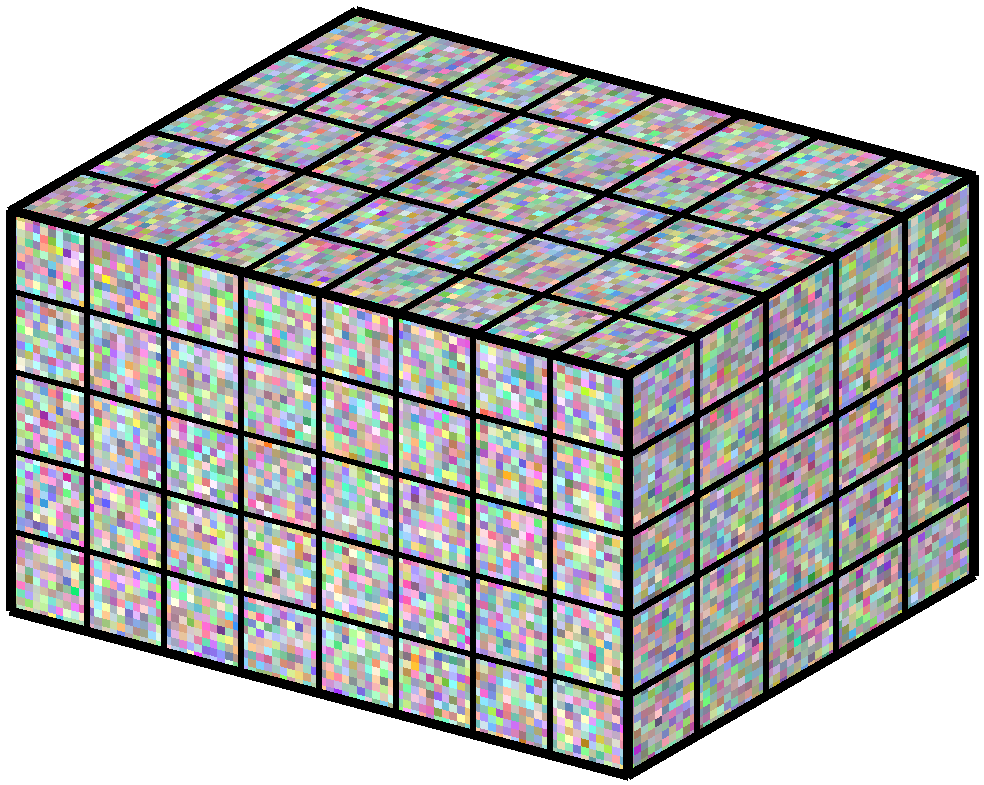
\includegraphics[width=2.2cm]{figures/generated/noise_cube.png}};
\node[sublbl, right=2pt of noisecube] {$\mathcal{N}(0, I)_{C:H}$};
\draw[arr] (noisecube.south) -- (ditbox.north);

\node[module, fill=corange!10, draw=corange!40, text=corange!60!black,
      minimum width=5.5em, minimum height=1.4em, font=\tiny\sffamily\bfseries]
    (adaln1) at ($(ditbox.north)+(0, -1.1)$) {AdaLN};
\node[module, fill=corange!25, draw=corange!50, text=corange!60!black,
      minimum width=5.5em, minimum height=1.4em, font=\tiny\sffamily\bfseries,
      below=0.1cm of adaln1]
    (dit1) {Self-Attention};
\node[module, fill=corange!10, draw=corange!40, text=corange!60!black,
      minimum width=5.5em, minimum height=1.4em, font=\tiny\sffamily\bfseries,
      below=0.1cm of dit1]
    (adaln2) {AdaLN};
\node[module, fill=corange!25, draw=corange!50, text=corange!60!black,
      minimum width=5.5em, minimum height=1.4em, font=\tiny\sffamily\bfseries,
      below=0.1cm of adaln2]
    (dit2) {Cross-Attention};
\node[module, fill=corange!10, draw=corange!40, text=corange!60!black,
      minimum width=5.5em, minimum height=1.4em, font=\tiny\sffamily\bfseries,
      below=0.1cm of dit2]
    (adaln3) {AdaLN};
\node[module, fill=corange!25, draw=corange!50, text=corange!60!black,
      minimum width=5.5em, minimum height=1.4em, font=\tiny\sffamily\bfseries,
      below=0.1cm of adaln3]
    (dit3) {Feedforward};

\node[sublbl, below=2pt of ditbox] {$\times N$};

%% ── Output PCA stack (right of DiT, 1/3 down) ──
\coordinate (pcaoutbase) at ([xshift=1.4cm]ditbox.east |- pca0);
\foreach \i/\file in {0/pca_ctx_t0, 1/pca_ctx_t4, 2/pca_fut_t0, 3/pca_fut_t15} {
    \node[imgframe] at ($(pcaoutbase)+(\i*2pt, -\i*2pt)$)
        (pcaout\i) {\includegraphics[width=2.2cm, interpolate=false]{figures/generated/\file.png}};
}
\node[sublbl] (futlbl) at ($(pcaout0.north)!0.5!(pcaout3.north)+(0, 12pt)$) {\textbf{Future Latents} $(\hat{\mathbf{z}}_{C:H})$};
\draw[arr] (ditbox.east |- pcaout0) -- (pcaout0.west);

%% ── Action trajectory plot (below DiT output) ──
\node[inner sep=0pt, minimum width=2.2cm, anchor=east] (actplot) at (pcaout3.east |- dit2) {%
    \tikz[baseline=-0.1em]{
        \draw[black!70, semithick, -{Stealth[length=2pt]}] (0,0) -- (0, 1.2);
        \draw[black!70, semithick, -{Stealth[length=2pt]}] (0,0) -- (2.1, 0);
        \draw[cblue, semithick] plot[smooth, tension=0.6] coordinates
            {(0,0.33) (0.35,0.53) (0.7,0.47) (1.05,0.73) (1.4,0.67) (1.75,0.77) (2.0,0.87)};
        \draw[corange, semithick] plot[smooth, tension=0.6] coordinates
            {(0,0.8) (0.35,0.67) (0.7,0.87) (1.05,0.53) (1.4,0.33) (1.75,0.4) (2.0,0.47)};
        \draw[cgreen, semithick] plot[smooth, tension=0.6] coordinates
            {(0,0.53) (0.35,0.2) (0.7,0.33) (1.05,0.4) (1.4,0.53) (1.75,0.27) (2.0,0.2)};
        \draw[cpurple, semithick] plot[smooth, tension=0.6] coordinates
            {(0,0.13) (0.35,0.33) (0.7,0.67) (1.05,0.33) (1.4,0.47) (1.75,0.6) (2.0,0.67)};
        \draw[cred, semithick] plot[smooth, tension=0.6] coordinates
            {(0,0.93) (0.35,0.8) (0.7,0.53) (1.05,0.67) (1.4,0.87) (1.75,0.8) (2.0,0.73)};
        \draw[cblue!60!black, semithick] plot[smooth, tension=0.6] coordinates
            {(0,0.47) (0.35,0.4) (0.7,0.2) (1.05,0.13) (1.4,0.2) (1.75,0.27) (2.0,0.33)};
    }%
};
\node[sublbl, anchor=east] (actlbl) at (futlbl.east |- actplot.north) {\textbf{Actions} $(\hat{\mathbf{a}}_{C:H})$};
\draw[arr] (ditbox.east |- actplot) -- (actplot.west);

%% ── VLM Block & State Input ──

%% Text input
\node[sublbl, below=0.3cm of c1f2] (textlbl) {\textbf{Text} $(\mathbf{l}_{C-1})$};
\node[draw, rounded corners=2pt, fill=cpurple!8, draw=cpurple!40,
      font=\tiny\sffamily, align=center,
      text width=1.1cm, minimum height=1.1cm, inner sep=0pt,
      below=2pt of textlbl]
    (textinput)
    {\textit{``pick up the red block...''}};

%% Proprioceptive State input
\node[sublbl, below=0.15cm of textinput] (statelbl) {\textbf{State} $(\mathbf{s}_{C-1})$};
\node[imgframe, below=2pt of statelbl] (stateinput)
    {
\includegraphics[width=0.9cm]{figures/robotic-arm.png}};

%% VLM Block (single, with xN, centered on cross-attention)
\node[module, fill=cpurple!25, draw=cpurple!50!black, text=cpurple!60!black,
      minimum width=7em]
    (vlmblock) at (vjepa.center |- dit2) {VLM Block};
\node[anchor=north east, inner sep=2pt] at (vlmblock.north east) {\snowflake[0.14]};
\draw[arr] ($(vlmblock.south east)+(-0.15, 0)$) -- ++(0, -0.35) coordinate (loopbot) -- ($(vlmblock.south west)+(0.15, -0.35)$) -- ($(vlmblock.south west)+(0.15, 0)$);
\node[sublbl, below=1pt of loopbot] {$\times N$};

%% Input fork (text + video to VLM)
\coordinate (vlmfork) at (vidfork |- vlmblock);
\draw[semithick, dotted] (vidfork) -- (vlmfork);
\draw[semithick, dotted] (textinput.east) -- ++(0.25, 0) |- (vlmfork);
\draw[arr, dotted] (vlmfork) -- (vlmblock.west);

%% Oplus: merge VLM + state before cross-attention
\coordinate (oplus_pos) at ($(pca3.east)!0.5!(ditbox.west)$);
\node[op, inner sep=0pt] (condoplus) at (oplus_pos |- dit2) {$\oplus$};
\draw[arr] (vlmblock.east) -- node[sublbl, above=1pt] {\textbf{Hidden State} $(\mathbf{h}_{i \in [1, N]})$} (condoplus.west);
\draw[semithick] (stateinput.east) -- (condoplus |- stateinput);
\draw[arr] (condoplus |- stateinput) -- (condoplus.south);
\draw[arr] (condoplus.east) -- (dit2.west);

\end{tikzpicture}
